\chapter{Аналитическая часть}
В данном разделе будут рассмотрены три алгоритма сортировок: сортировка вставками, сортировка выбором, ее улучшение --- пирамидальная сортировка и битонная сортировка.
\section{Сортировка вставками}

Суть алгоритма заключается в следующем: на каждом  шаге  алгоритма  выбирается один  из  элементов входных данных и  помещается  на нужную  позицию  в  уже  отсортированной последовательности до тех  пор,  пока  набор  входных  данных  не будет  исчерпан.
Алгоритму  необходимо  для  каждого нового  элемента  выбрать нужное место для вставки в уже упорядоченный массив данных, так что элементы  входной  последовательности просматриваются  по одному,  и каждый новый поступивший элемент размещается  в  подходящее  место среди  ранее  упорядоченных  элементов.

\section{Сортировка выбором}

Алгоритм сортировки выбором заключается в поиске на необработанном срезе массива или списка минимального значения и в дальнейшем обмене этого значения с первым элементом необработанного среза. На следующем шаге необработанный срез уменьшается на один элемент.

Шаги выполнения алгоритма:
\begin{enumerate}
	\item Находим  минимальный (максимальный)  элемент  в  текущем  массиве.
	\item Производим обмен этого элемента со значением первой неотсортированной позиции.  Обмен  не  нужен,  если минимальный (максимальный) элемент уже находится на данной позиции.
	\item Сортируем оставшуюся часть массива, исключив из рассмотрения уже отсортированные элементы.
\end{enumerate}

\subsection{Пирамидальная сортировка}

Пирамидальная сортировка (англ. Heap Sort) предложена в 1964 году Дж. Уильямсом. Основана на использовании бинарного сортирующего дерева (пирамиды) и базируется на сортировке выбором, по сути является его усовершенствованием~\cite{book_lipachev, book_sort_algorithms, book_knut, book_kormen}.

Пирамида (англ. binary heap) определяется как структура данных, представляющая собой объект-массив, который можно рассматривать как почти полное бинарное дерево.
Каждый узел этого дерева соответствует определенному элементу массива.
На всех уровнях, кроме последнего, дерево полностью заполнено (заполненным считается уровень, который содержит максимально возможное количество узлов).
Последний уровень заполняется слева направо до тех пор, пока в массиве не закончатся элементы.

В пирамиде, представленной на рисунке \ref{fig:heap_structs}, число в окружности, представляющей каждый узел дерева, является значением, сортируемым в данном узле. Число над узлом — это соответствующий индекс массива. Линии, попарно соединяющие элементы массива, обозначают взаимосвязь вида “родитель-потомок”. Родительские элементы всегда расположены слева от дочерних. Данное дерево имеет высоту, равную 3; узел с индексом 4 (и значением 8) расположен на первом уровне.

\begin{figure}[h]
	\centering
	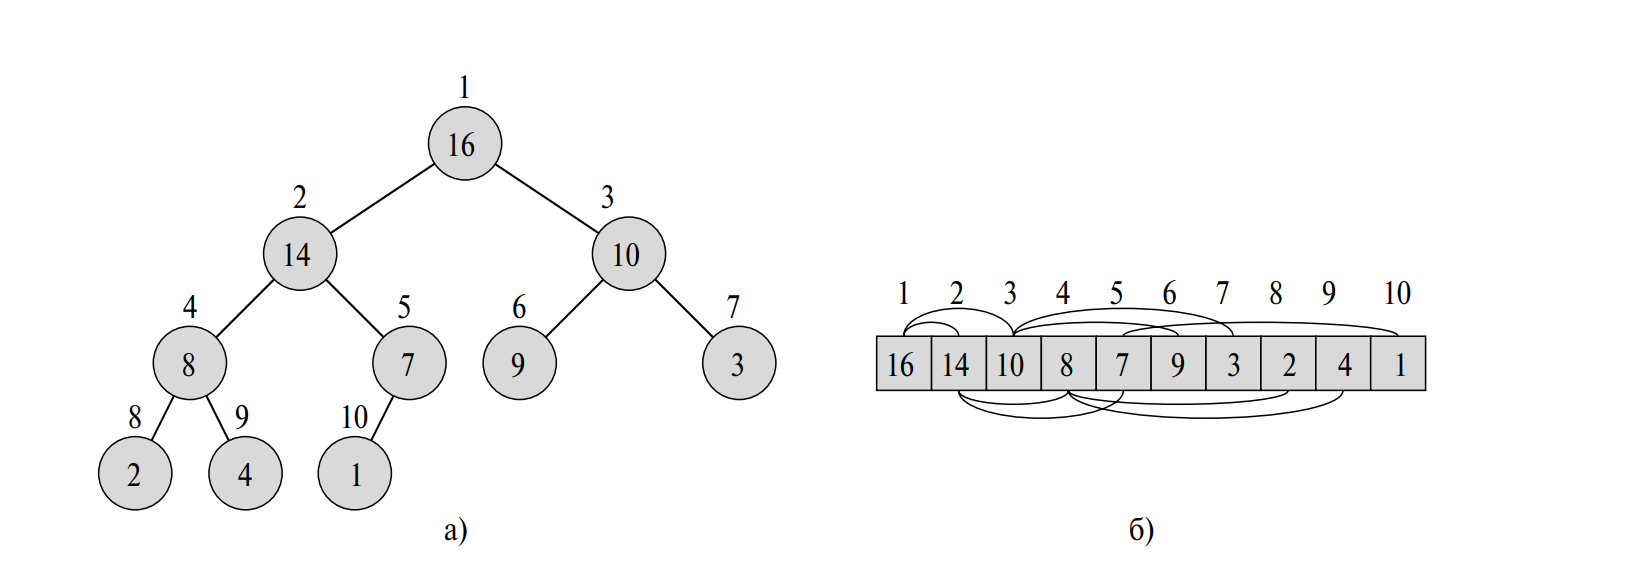
\includegraphics[height=0.25\textheight]{img/heap_structs.png}
	\caption{Пирамида, представленная в виде a) бинарного дерева и б) массива}
	\label{fig:heap_structs}
\end{figure}

Обозначим следующие особенности:
\begin{enumerate}
	\item родительский элемент в массиве будет находится под индексом - $\frac{i}{2}$;
	\item правый потомок в массиве будет находится под индексом - $2 \cdot i$;
	\item левый потомок в массиве будет находится под индексом - $2 \cdot i + 1$.
\end{enumerate}

Различают два вида бинарных пирамид: неубывающие и невозрастающие.
В пирамидах обоих видов значения, расположенные в узлах, удовлетворяют свойству пирамиды (heap property), являющемуся отличительной чертой пирамиды того или иного вида.
Свойство невозрастающих пирамид (max-heap property) заключается в том, что для каждого отличного от корневого узла с индексом $i$ выполняется следующее неравенство:

\begin{equation}
	A[i / 2] \geq A[i].
\end{equation}

Другими словами, значение узла не превышает значение родительского по отношению к нему узла. Таким образом, в невозрастающей пирамиде самый большой элемент находится в корне дерева, а значения узлов поддерева, берущего начало в каком-то элементе, не превышают значения самого этого элемента. Принцип организации неубывающей пирамиды (min-heap) прямо противоположный. Свойство неубывающих пирамид (min-heap property) заключается в том, что для всех отличных от корневого узлов с индексом $i$ выполняется такое неравенство:

\begin{equation}
	A[i / 2] \leq A[i].
\end{equation}

Таким образом, наименьший элемент такой пирамиды находится в ее корне.

\section{Битонная сортировка}

Битонная сортировка (англ. Bitonic sorter) — параллельный алгоритм сортировки данных, метод для создания сортировочной сети. Разработан американским информатиком Кеннетом Бэтчером в 1968 году.

Идея данного алгоритма заключается в том, что исходный массив преобразуется в битонную последовательность --- последовательность, которая сначала возрастает, а потом убывает.
Ее можно эффективно отсортировать следующим образом: разбить массив на две части, создадь два массива, в первый добавить все элементы, равные минимуму из соответственных элементов каждой из двух частей, а во второй --- равные максимуму.
В результате получатся две битонные последовательности, каждую из которых можно рекурсивно отсортировать тем же образом, после чего можно объединить два массива (так как любой элемент первого меньше или равен любого элемента второго).
Для того, чтобы преобразовать исходный массив в битонную последовательность, можно сделать следующее: если массив состоит из двух элементов, можно просто завершить выполнение, иначе нужно разделить массив пополам, рекурсивно вызвать от половин массива алгоритм, после чего отсортировать первую часть по порядку, вторую в обратном порядке и объединить их.
В результате получается битонная последовательность.

Также важно заметить, что размер массива должен быть равен степени двойки.
\section*{Вывод}
В данном разделе были рассмотрены алгоритмы сортировки - битонная, пирамидальная и вставками.
Рассмотренные сортировки следует реализовать, изучить трудоемкость и проанализировать время, необходимое для выполнения.
